\documentclass[dvisvgm,tikz,margin=2pt]{standalone}
\usepackage{amsmath,amssymb,amsthm,mathtools}
\usepackage{tikz}
\usetikzlibrary{positioning,calc}
\usepackage{xcolor}
\newcommand{\R}{\mathbb{R}}
\newcommand{\Q}{\mathbb{Q}}
\newcommand{\abs}[1]{\lvert #1\rvert}
\newcommand{\norm}[1]{\lVert #1\rVert}
\newcommand{\RSSP}{\textsc{Riesz-Subset}}
\newcommand{\MIS}{\textsc{Independent-Set}}
\newcommand{\sgnspin}{\{-1,+1\}}
\begin{document}
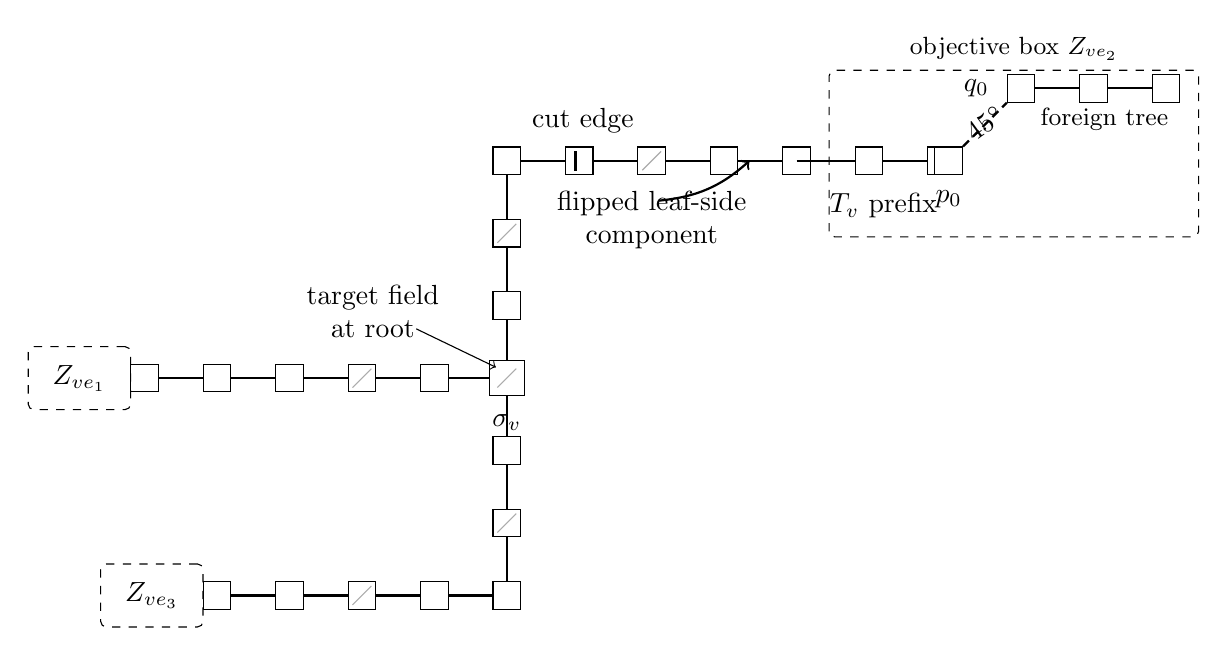
\begin{tikzpicture}[x=0.92cm,y=0.92cm]
  % Styles local to this figure.
  \tikzset{
    sel/.style={draw,minimum size=4.5mm,inner sep=0pt,fill=white},
    smallsel/.style={draw,minimum size=3.5mm,inner sep=0pt,fill=white},
    obj/.style={draw,dashed,rounded corners=2pt,inner sep=4pt},
    wire/.style={thick},
    aux/.style={gray!65}
  }

  % Root and main three-arm tree.
  \node[sel] (r) at (0,0) {};
  \node[below=3pt of r] {$\sigma_v$};

  \draw[wire] (r) -- (-5,0);
  \draw[wire] (r) -- (0,3) -- (4,3);
  \draw[wire] (r) -- (0,-3) -- (-4,-3);

  % Unit selector centers, schematic but evenly spaced.
  \foreach \x in {-1,-2,-3,-4,-5} {\node[smallsel] at (\x,0) {};}
  \foreach \y in {1,2,3} {\node[smallsel] at (0,\y) {};}
  \foreach \x in {1,2,3,4} {\node[smallsel] at (\x,3) {};}
  \foreach \y in {-1,-2,-3} {\node[smallsel] at (0,\y) {};}
  \foreach \x in {-1,-2,-3,-4} {\node[smallsel] at (\x,-3) {};}

  % Small diagonal marks in representative selectors.
  \draw[aux] (-0.13,-0.13) -- (0.13,0.13);
  \draw[aux] (-2.13,-0.13) -- (-1.87,0.13);
  \draw[aux] (-0.13,1.87) -- (0.13,2.13);
  \draw[aux] (1.87,2.87) -- (2.13,3.13);
  \draw[aux] (-0.13,-2.13) -- (0.13,-1.87);
  \draw[aux] (-2.13,-3.13) -- (-1.87,-2.87);

  % Two schematic objective terminals.
  \node[obj,minimum width=1.3cm,minimum height=0.8cm] at (-5.9,0) {$Z_{ve_1}$};
  \node[obj,minimum width=1.3cm,minimum height=0.8cm] at (-4.9,-3) {$Z_{ve_3}$};

  % Detailed upper-right objective box.
  \draw[obj] (4.45,1.95) rectangle (9.55,4.25);
  \node[font=\small] at (7.0,4.55) {objective box $Z_{ve_2}$};
  \draw[wire] (4,3) -- (6.1,3);
  \foreach \x in {5,6} {\node[smallsel] at (\x,3) {};}
  \node[smallsel] (p0) at (6.1,3) {};
  \node[below=2pt of p0] {$p_0$};

  \node[smallsel] (q0) at (7.1,4) {};
  \node[left=3pt of q0] {$q_0$};
  \draw[wire] (q0) -- (9.1,4);
  \foreach \x in {8.1,9.1} {\node[smallsel] at (\x,4) {};}
  \draw[densely dashed,thick] (p0) -- (q0);
  \node[rotate=36] at (6.60,3.52) {$45^\circ$};
  \node[below] at (5.2,2.68) {$T_v$ prefix};
  \node[font=\small] at (8.25,3.58) {foreign tree};

  % Example component cut and leaf-side component annotation.
  \draw[very thick] (0.95,2.86) -- (0.95,3.14);
  \node[above] at (1.05,3.25) {cut edge};
  \draw[->,thick] (2.1,2.45) to[bend right=18] (3.35,3.0);
  \node[align=center] at (2.0,2.18) {flipped leaf-side\\component};

  % Field annotation.
  \draw[->] (-1.25,0.68) -- (-0.15,0.15);
  \node[align=center] at (-1.85,0.92) {target field\\at root};
\end{tikzpicture}
\end{document}
